\documentclass[11pt,english,a4paper]{book}
\usepackage{../futhark} %I denne filen har vi alt av \usepackage, alle egendefinerte kommandoer osv.

\begin{document}

%Forside:
	\thispagestyle{empty}   %Ingen sidetall
	\forsideRapport		%Denne setter inn forsiden.
	\clearpage		%Ny side
	
%Sammendrag og forord:
	\pagestyle{plain}	%Stil på sammendrag og forord.
	\pagenumbering{roman} 	%Sidetall på formen i, ii, osv. på sammendrag, forord og innholdsfortegnelse.

	\sammendragEn{Text in abstract}
	%\coffee{4}
	\forordEn{Text in foreword}
	%\coffee{1}
	\clearpage		%Ny side

%Innholdsfortegnelse (automagisk)
	\tableofcontents
	\clearpage		%Blank side
	\thispagestyle{empty}	%Uten sidetall

%Kapitler:
	\kapittelstil %Fikser stilen i kapitlene

<<<<<<< HEAD
	\chapter{Introduction}
%In this chapter, we don't need numbering of subsections (there are none).
\setcounter{secnumdepth}{1}

\section{Problem formulation}
The problem considered in this project is the preparation of bacon in a microwave oven. Bacon is
defined as cured meat from side and back cuts of a pig. A microwave oven in this context is a
household appliance typically delivering 750 W of microwave effect at a frequency of 2.1 GHz
to a Faraday cage of volume 40 liters. 

The motivation for the problem formulation was clear. As soon as modeling of food preparation was
brought on the table, bacon seemed a prime choice. A microwave oven may seem an odd choice for
bacon, but previous experiments have shown that optimal bacon can consistently be attained with this
preparation method. Obvious advantages over traditional bacon preparation include less cleaning up
to do afterwards and a shorter time-to-plate. The caveat is that microwave preparation is less
suitable for feedback during the cooking process, as the bacon is obscured from view. To the
traditional bacon chef, used to a touch-and-go approach, this is an obstacle to implementation, as
overcooking bacon in a microwave oven yields inedible results. The
purpose of this work, then, is to establish reliable numerical simulations that can serve as a basis
for estimating cooking time for an arbitrary slice of bacon.

As the project considers the optimal preparation of bacon in a microwave oven, two natural questions
were formulated:

\begin{itemize}
  \item How is preparation of bacon in a microwave oven modelled numerically?
  \item How does the size of the bacon affect the preparation, and what preparation time is optimal?
\end{itemize}

\section{Reasoning behind the problem formulation}
The first question is obvious, as any attempt at predicting the preparation time necessitates a
numerical model of bacon in a microwave oven; a simple glance at the relevant
equations tells the experienced numerics person that no analytical solution
exists. With a numerical solution of the heat and mass transport equations, the
optimal preparation time can be predicted. But this presumes an understanding of
what makes good bacon. So what does?

Work done by \cite{intarwebz} and \cite{maillard} suggest that two factors are important in
determining good bacon. The first is a high enough temperature that the Maillard
reaction can take place, which happens around 140$^{circ}$C. The second is that
a significant proportion of the fat has melted and has been transported out of
the bacon. Both of these factors are naturally affected by the composition of
the bacon; especially water and fat content will play a major role.

Having identified these two factors as the important criteria for an optimal
solution, experimental work is needed to determine the correlation between
temperature and fat loss, and how finished bacon is. This is, of course, also a
subjective question - different people prefer different grades of crispness.

Another experimental question is how much of the microwave effect that is
absorbed by the bacon. The second law of thermodynamics dictates that some of
the effect is lost in the microwave magnetron, the question is how much effect
is dissipated in the bacon. This may include losses besides that of the
magnetron, which has a typical efficiency of 65\% \cite{namba}. It turns out
that common household microwave ovens are rated to include this loss,
with standardized calibration procedures published by the IEC's SC 59K, so a 750 W
microwave oven will typically draw 1.1 kW of electrical power from the mains
socket. This means using the rated power will be good enough for our purposes.

Finally, experiments are needed to verify the accuracy of the numerical results.
As heat and mass transport is a Complicated Problem, this is not guaranteed a
priori.

%Reset secnumdepth for other chapters
\setcounter{secnumdepth}{2}
 	%Kap. 1
	\chapter{Theory}
\section{The physical system}
The physical system to be modeled is a thin, rectangular strip of bacon which is
subjected to approx. 750 watts of microwave radiation at the frequency of 2.4
GHz. To be modeled is the heat in the strip, phase transitions and transport.

\section{Our approach}
\begin{figure}[!h]
  \begin{center}
    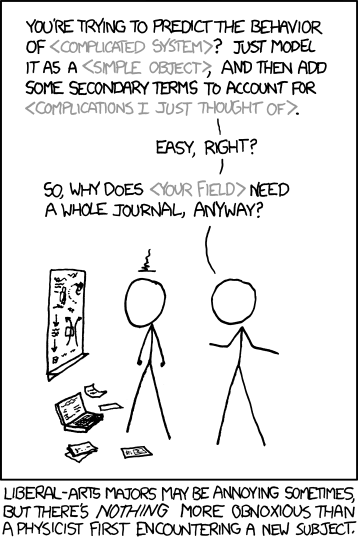
\includegraphics[width=0.4\linewidth]{physicists.png}
  \end{center}
  \caption{Our initial approach to the problem}
  \label{fig:xkcd_physics}
\end{figure}

Initially, our approach to modelling was to use a staggered approach: first solve the
heat equation for the three media meat, solid fat, and liquid fat, thus giving
the temperature at step $n$. Then at step $n+1$, the temperature is regarded as
known, and we solve the transport equation for liquid fat out of the bacon. Then
we know the distribution of liquid fat at step $n+2$, where we solve the heat
equations again, and we repeat ad nauseam.

\section{The heat equations}
The differential equations governing the heat transport are all variations of the heat
equation, with various source terms, \cref{eq:temp}:
\begin{align}
  \label{eq:temp}
  (\rho c_p)_m \pd{T}{t} - \alpha_m \grad{^2 T} &= J^{MW} \quad \rm{m,} \\
  \eta_s (\rho c_p)_s \pd{T}{t} - \eta_s\alpha_s \grad{^2 T} &= J^{MW} - J^{Melt}  \quad \rm{s,} \\
  \eta_l (\rho c_p)_l \pd{T}{t} - \eta_s\alpha_l \grad{^2 T} - \eta_l(\rho c_p)_l(\v{v}\cdot
  \grad{})T &= J^{MW}  \quad \rm{l.}
\end{align}
Here the subscript $m$ denotes meat, $s$ denotes solid fat, and $l$ denotes
liquid fat. $J^{MW}$ is the source term representing the microwave oven.
In the initial approach, this is modelled as a cylindrically symmetric term,
with the radial power distribution on the form \cref{eq:effektfordeling},
\begin{equation}
  J^{MW}(r) = 0.5 + 2.55008x - 0.588013x^2 + 0.032445x^3 + 0.00124411x^4 - 0.0000973516x^5 \rm{,}
  \label{eq:effektfordeling}
\end{equation}
i.e. a fifth degree polynomial, interpolated from the results in \cite{huang+zhu}.

Furthermore, there is the term $J^{Melt}$ which represents heat loss due to
latent heat in the solid-liquid phase transition. This can be written as 
\[ \frac{L \rho}{T_2-T_1} \pd{T}{t} \rm{,} \quad T \in (T_1,T_2) \rm{,}\]
where the fat is melting between the temperatures $T_1$ and $T_2$. For fat these
are typically around 30-50$^\circ$C. For $T \notin (T1,T2)$ this term is zero,
and it is readily seen that this is equivalent to a modification of the constant
$c_{p,l}$ in \cref{eq:temp} when $T \in (T1,T2)$, thus it is not a serious
complication.

In the last of the heat equations, there also appears what is called a
convective derivative, on the form $(\v{v}\cdot \grad{})T$. This is a somewhat
more complicated term, and is essentially a modification due to transport of
liquid fat implying an implicit transport of heat. However, in the staggered
approach used here, the velocity field is considered as known when it comes to
the heat equations.

\section{The transport equations}







		%Kap. 2
	\chapter{Numerics}

\section{Numerical schemes}

In this project we have use the Cranch-Nicholson method to discretize the heat
equation \cref{eq:temp} in 3D over a finite grid. The Crank-Nicholson method is based on the equation \cref{integral}, where the trapezoidal rule \cref{trapezoidalrule} is used to approximate the integral on the right hand side. We insert the right hand side of the heat equation in the resulting expression \cref{res}, and use Taylor-expansion to obtain the discretizaion. We use the notation \cref{notations} in the rest of the document.
\begin{equation}
\partial_{x}^{k}u=\frac{\partial^{k}u}{\partial^{}x^{k}},\quad \quad \partial_{t}^{k}u=\frac{\partial^{k}u}{\partial^{}t^{k}} \quad \quad u_{m}^{n+\alpha k } = u(x_{m},t_{n}+\alpha k)
\label{notations}
\end{equation}

\begin{equation}
u(x_m,t_{n+1}) - u(x_m,t_n) = \int_{t_n} ^{t_{n+1}} u_t(x_m,t) dt
\label{integral}
\end{equation}

\begin{equation}
\int_0^k f(t) dt = \frac{1}{2} k (f(0) - f(k)) -\frac{1}{12} k^3 f''(\frac{k}{2}) + ...
\label{trapezoidalrule}
\end{equation}
We thus obtain
\begin{eqnarray}
\label{res}
u_m^ {n+1} &=& u_m^ n + \frac{1}{2} k(\partial_t u_m^n + \partial_t u_m^{n+1}) - \frac{1}{12} k^3 \partial_t ^3 u_m^{n+\frac{1}{2}} \\
&\stackrel{\text{\tiny heat eq.}}{=}& u_m^ n + \frac{1}{2} k(\partial_x^2 u_m^n + \partial_y^2 u_m^n + \partial_z^2 u_m^n + \partial_x^2 u_m^{n+1} + \partial_y^2 u_m^{n+1} + \partial_z^2 u_m^{n+1}) - \frac{1}{12} k^3 \partial_t ^3    u_m^{n+\frac{1}{2}} \nonumber
\end{eqnarray}
Using central differences \cref{centraldiff}, and denoting the step sizes in $x, y, z$ direction by $h, f, g$ respectively, gives
\begin{eqnarray*}
u_m^{n+1} &=& u_m^ n + \frac{1}{2} k(\frac{1}{h^2}\delta_x^2 u_m^n + \frac{1}{f^2}\delta_y^2 u_m^n + \frac{1}{g^2}\delta_z^2 u_m^n + \frac{1}{h^2}\delta_x^2 u_m^{n+1} + \frac{1}{f^2}\delta_y^2 u_m^{n+1} + \frac{1}{g^2}\delta_z^2 u_m^{n+1}) \\
  &&- \frac{1}{2} k (\frac{1}{12}h^2\partial_x^4 u_m^n + \frac{1}{12}g^2\partial_y^4 u_m^n + \frac{1}{12}f^2\partial_z^4 u_m^n + \frac{1}{12}h^2\partial_x^4 u_m^{n+1} + \frac{1}{12}g^2\partial_y^4 u_m^{n+1} + \frac{1}{12}f^2\partial_z^4 u_m^{n+1} + ...) \\
  &&- \frac{1}{12} k^3 \partial_t ^3 u_m^{n+\frac{1}{2}} \\ 
  %&=& u_m^n + \frac{r}{2}(\delta_x^2 u_m^n + \delta_x^2 u_m^{n+1}) + \frac{p}{2}(\delta_y^2 u_m^n + \delta_y^2 u_m^{n+1}) + \frac{q}{2}(\delta_z^2 u_m^n + \delta_z^2 u_m^{n+1}) + \tau_m^n
\end{eqnarray*}
where
\begin{equation}
\delta_{r}^{2}U_m^{n}=\frac{U_{m+1}^{n}-2U_m^{n}+U_{m-1}^{n}}{{\Delta r}^{2}}
\label{centraldiff}
\end{equation}
We thus obtain the implicit method for the heat equation
\begin{equation}
u_m^{n+1}-k(\frac{1}{h^2}\delta_x^2 u_m^{n+1}-\frac{1}{f^2}\delta_y^2 u_m^{n+1}-\frac{1}{g^2}\delta_z^2 u_m^{n+1})=u_m^n + k(\frac{1}{h^2}\delta_x^2 u_m^n + \frac{1}{f^2}\delta_y^2 u_m^n +\frac{1}{g^2}\delta_z^2 u_m^n)
\label{crank}
\end{equation}
with truncation error error
\begin{eqnarray}
\frac{\tau_m^ n}{k} &=& -\frac{1}{12} k^2 \partial_t^2 u_m^{n+\frac{1}{2}} - \frac{1}{12} h^2 \partial_x^4 u_m^{n+\frac{1}{2}} - \frac{1}{12} g^2 \partial_y^4 u_m^{n+\frac{1}{2}} - \frac{1}{12} f^2 \partial_z^4 u_m^{n+\frac{1}{2}}\\
&=& O(k^2 + h^2 + g^2 + f^2)
\label{truncerror}
\end{eqnarray}

Here we have used that $\frac{1}{2}(\partial_x^4 u_m^n + \partial_x^4 u_m^{n+1}) = \partial_x^4 u_m^{n+\frac{1}{2}} + O(k^2)$. 
The truncation error $\tau_m^n \Rightarrow 0$ as $h,f,g,k \Rightarrow 0$, and the Crank-Nicholson method is consistent for the heat equation. To see if the method converges we perform a von Neumann analysis of the numerical scheme.

\section{Von Neumann analysis of the Crank-Nicholson-scheme}

The von Neumann analysis is based on Fourier analysis. The method consist of substituting 
\begin{equation*}
	U_m^n=\xi^n e^{i \beta x_m} \quad \quad  i=\sqrt{-1}
\end{equation*}
in the difference equation and solve for $\xi$.
For the method to be stable it has to meet the condition
\begin{equation}
	\mid{\xi}\mid \leq 1
	\label{stabcond}
\end{equation}

Here we only perform the Neumann analysis for the one-dimensional heat equation problem. We thus obtain the expression
\begin{equation*}
\xi^{n+1} e^{i\beta x_{j}} = \xi^{n} e^{i\beta x_j}\left(1-2D\right) + \xi^{n+1}D\left(e^{i\beta x_{j+1}} - 2e^{i\beta  x} + e^{i\beta x_{j-1}}\right) + \xi^{nD}\left(e^{i\beta x_{j+1}} + e^{i\beta x_{j-1}}\right)
\end{equation*}

where
\begin{equation*}
D = \frac{1}{2}\frac{\alpha\Delta t}{(\Delta x)^2}
\label{eq:crank-D}
\end{equation*}
\marginpar{A typical
\textbf{C}ourant-\textbf{F}riedrichs-\textbf{L}ewy condition is an inequality of the form
$\frac{\Delta t}{\Delta x} < C$, with C a constant. }
%Marginpar makes a note in the margin, e.g. for explaining things.

Dividing  by $\xi^ne^{i\beta x_j}$, and using $x_{j+1} = x_j + h$ one obtains    %\href{eq:crank-D}
\begin{eqnarray*}
\xi\left[1-D\left(2\cos{\beta h} - 2\right)\right] &=& 1 - 2D\left(1-\cos{\beta h}\right) \\
\cos{\beta h} &=& 1-2\sin^2{\frac{\beta h}{2}} \\
\xi\left(1+4D\sin^{2}{\frac{\beta h}{2}}\right) &=& 1 - 4D\sin^2{\frac{\beta h}{2}} \\
\xi &=& \frac{1-4D\sin^2{\frac{\beta h}{2}}}{1+4D\sin^2{\frac{\beta h}{2}}}
\end{eqnarray*}
As the maximum value of $\sin^2{x}$ is 1, the methods meets the stability condition \ref{stabcond}.
\begin{equation}
|\xi | = \left|\frac{1-4D}{1+4D}\right|
\end{equation}

Since D always are positiv, we get that the Crank-Nicolson
scheme for the heat equation is \emph{unconditionally stable}. In practice it may happen that the method oscillates if the time steps and space steps do not fulfill a CFL-condition.
\\
\\
From Lax' equivalent theorem, which state that a consistent difference scheme will converges if and only if it is stable, the Crank-Nicholson scheme will converge.


\section{Truncation error in the Crank-Nicolson scheme}

The Crank-Nicholson method is based on the trapezoidal rule. From the trapezoidal rule the truncation error is represented by
\begin{equation*}
\int_0^k f(t) dt = \frac{1}{2} k (f(0) - f(k)) -\frac{1}{12} k^3 f''(\frac{k}{2}) + ...
\end{equation*}
Using the formula
\begin{equation*}
	u(x_m,t_{n+1}) - u(x_m,t_n) = \int_{t_n} ^{t_{n+1}} u_t(x_m,t) dt
\end{equation*}
and approximating the integral by the trapezoidal rule, and abbreviate the notation $u_m^{n+1/2} = u(x_m,t_n+\frac{1}{2} k)$, one obtain
\begin{eqnarray*}
u_m^ {n+1} &=& u_m^ n + \frac{1}{2} k(\partial_t u_m^n + \partial_t u_m^{n+1}) - \frac{1}{2} k^3 \partial_t ^3 u_m^{n+\frac{1}{2}} \\
		   &\stackrel{\text{\tiny heat eq.}}{=}&  u_m^ n + \frac{1}{2} k(\partial_x^2 u_m^n + \partial_y^2 u_m^n + \partial_z^2 u_m^n + \partial_x^2 u_m^{n+1} + \partial_y^2 u_m^{n+1} + \partial_z^2 u_m^{n+1}) - \frac{1}{2} k^3 \partial_t ^3 u_m^{n+\frac{1}{2}}
\end{eqnarray*}
Discretizing the double derivative with central differences, and denoting the step sizes in $x, y, z$ direction by $h, f, g$ respectively, gives
\begin{eqnarray*}
u_m^{n+1} &=&  u_m^ n + \frac{1}{2} k(\frac{1}{h^2}\delta_x^2 u_m^n + \frac{1}{f^2}\delta_y^2 u_m^n + \frac{1}{g^2}\delta_z^2 u_m^n + \frac{1}{h^2}\delta_x^2 u_m^{n+1} + \frac{1}{f^2}\delta_y^2 u_m^{n+1} + \frac{1}{g^2}\delta_z^2 u_m^{n+1}) \\
 		  &&- \frac{1}{2} k (\frac{1}{12}h^2\partial_x^4 u_m^n + \frac{1}{12}g^2\partial_y^4 u_m^n \frac{1}{12}f^2\partial_z^4 u_m^n + \frac{1}{12}h^2\partial_x^4 u_m^{n+1} + \frac{1}{12}g^2\partial_y^4 u_m^{n+1} \frac{1}{12}f^2\partial_z^4 u_m^{n+1} ) \\
 		  &&- \frac{1}{2} k^3 \partial_t ^3 u_m^{n+\frac{1}{2}} \\
 		  &=& u_m^n + \frac{r}{2}(\delta_x^2 u_m^n + \delta_x^2 u_m^{n+1}) + \frac{p}{2}(\delta_y^2 u_m^n + \delta_y^2 u_m^{n+1}) + \frac{q}{2}(\delta_z^2 u_m^n + \delta_z^2 u_m^{n+1}) + \tau_m^n
\end{eqnarray*}
where $r = k/h^2$, $p = k/f^2$, $q = k/g^2$, and $\tau_m^n$ is the truncation error times $k$. The expression for $\tau_m^n$ is
\begin{equation*}
\tau_m^n = -\frac{1}{12} k^3 \partial_t^2 u_m^{n+\frac{1}{2}} - \frac{1}{12} k h^2 \partial_x^4 u_m^{n+\frac{1}{2}} - \frac{1}{12} k g^2 \partial_y^4 u_m^{n+\frac{1}{2}} - \frac{1}{12} k f^2 \partial_z^4 u_m^{n+\frac{1}{2}}
\end{equation*}
where we have used $\frac{1}{2}(\partial_x^4 u_m^n + \partial_x^4 u_m^{n+}) = \partial_x^4 u_m^{n+\frac{1}{2}} + O(k^2)$. Hence, the truncation error is 
\begin{eqnarray*}
\frac{\tau_m^ n}{k} &=& -\frac{1}{12} k^2 \partial_t^2 u_m^{n+\frac{1}{2}} - \frac{1}{12} h^2 \partial_x^4 u_m^{n+\frac{1}{2}} - \frac{1}{12} g^2 \partial_y^4 u_m^{n+\frac{1}{2}} - \frac{1}{12} f^2 \partial_z^4 u_m^{n+\frac{1}{2}}\\
					&=& O(k^2 + h^2 + g^2 + f^2)
\end{eqnarray*}

	%Kap. 3
	
\chapter{Implementation}

\section{Tools}

The programming language chosen to implemented the system was c++.
The arguments leading to this choice was:

\begin{itemize}
\item Most of the group members had some earlier experience with the language.
\item It allows for a high level of abstraction without losing control of the
underlying hardware.
\item The code can be easily parallellized for shared memory machines using OpenMP.
\item Many libraries exist for C++ that implement highly optimized linear algebra
functionality.
\end{itemize}

Other languages considered were Matlab and C.

The tool chosen to visualize the resulting data was gnuplot and ffmpeg. Writing a
program using OpenGL was considered, but dismissed on the grounds of beeing too time consuming.

\section{Program design}

\begin{figure}[!h]
  \begin{center}
    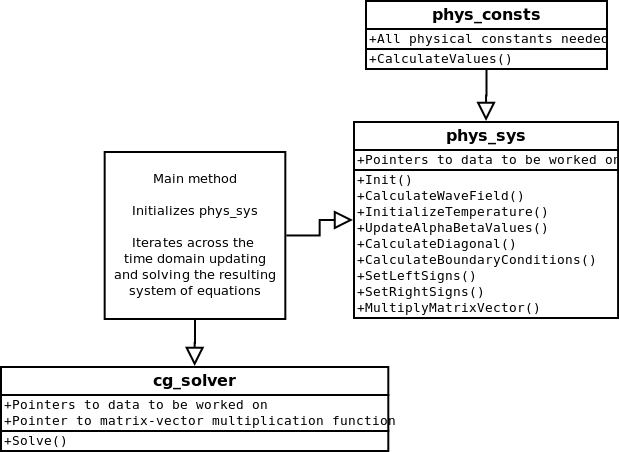
\includegraphics[width=0.5\linewidth]{classdiagram.png}
  \end{center}
  \caption{Class diagram of c++ implementation}
  \label{fig:classdiagram}
\end{figure}

The program mainly consist of three parts:

\begin{itemize}
\item C++ implementation of Linear algebra functionality of the discrete equations.
\item C++ implementation of the conjugate gradient method for solving the
equations described.
\item Bash script for generating plots and and movie of the generated data.
\end{itemize}

See \cref{fig:classdiagram} for a class diagram of c++ implementation.

The Bash script is not discussed in further detail as it can be considered to be
very simple.

See \cref{ap:source_code} for source code and scripts.

\section{The physical system}

The main task of the physical system is to implement a matrix-vector multiplication
procedure for the heat equation to be used in the conjugate gradient method, 
a method for calculating the heating properties of the microwave and a method 
for calculating the velocity of mass transfer.

\subsection{Partitioning of the problem}

The problem is to perform the multiplication of a sparse, symmetrix, matrix with a
vector. To describe this procedure we have vectors $a$, $b$ and $t$ containing alpha,
beta, and temperature values respectively. The alpha values represent the heat 
conduction properties, the beta values describe the substance's ability to be heated
by microwaves and the temperature values naturally contains the temperatures. We need
these vectors because each point in the grid contains a particular substance in
a particular phase.

\begin{figure}[!h]
  \begin{center}
    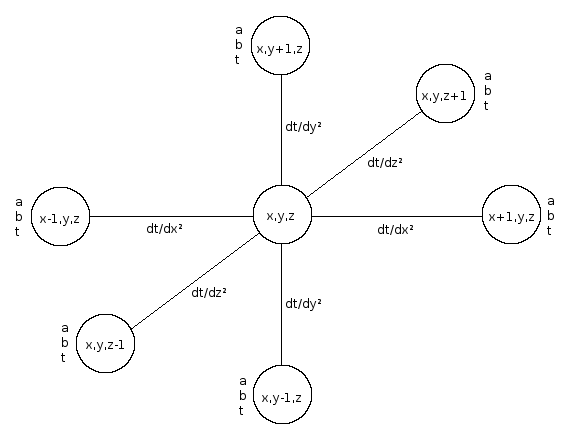
\includegraphics[width=0.5\linewidth]{stencil.png}
  \end{center}
  \caption{Stencil}
  \label{fig:stencil}
\end{figure}

\begin{figure}[!h]
  \begin{center}
    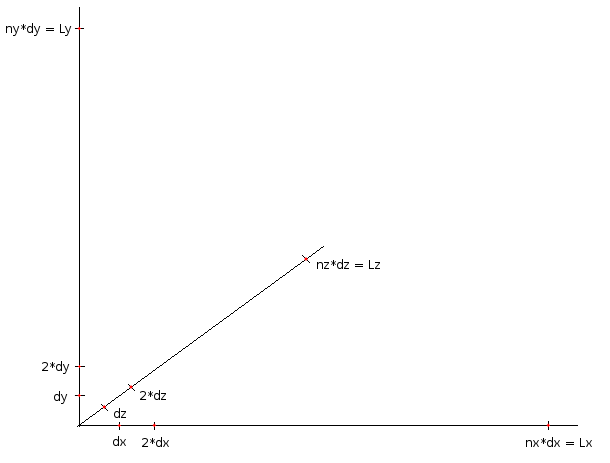
\includegraphics[width=0.5\linewidth]{grid.png}
  \end{center}
  \caption{Grid}
  \label{fig:grid}
\end{figure}

We say that position $j$ of the vectors is given by:
\begin{equation}
j = z*n_x*n_y + y*n_x + x
\end{equation}

where $n_x$, $n_y$, $n_z$ is the number of points in the $x$, $y$ and $z$ directions
respectively, and $x$, $y$ and $z$ is the points on the grid, See \cref{fig:grid} and
\cref{fig:stencil}

The center of the stencil, given by $j$ can be described by the equations:
\begin{eqnarray}
  x & \cong & j\%n_x \\
  y & \cong & (j/n_x)\%n_y \\
  z & \cong & j/n_x/n_y 
\end{eqnarray}

where $/$ and $ \% $ is the integer division and modulo operators respectively.

In addition to this, we define two more vectors and one more matrix:

The offset matrix represents the neighbours in the stencil (see \cref{fig:stencil}):
\begin{equation}
O =
\left[
\begin{array}{ccc}
0 & 0 & -1 \\
0 & -1 & 0 \\
-1 & 0 & 0 \\
0 & 0 & 0 \\
1 & 0 & 0 \\
0 & 1 & 0 \\
0 & 0 & 1 \\
\end{array}
\right]
\end{equation}

The delta vector representing the difference in time and distance used in the heat
equation:
\begin{equation}
D = \{ \frac{dt}{dz^2}, \frac{dt}{dy^2}, \frac{dt}{dx^2}, 0, \frac{dt}{dx^2}, \frac{dt}{dy^2}, \frac{dt}{dz^2} \}
\end{equation}

The vector containing the offsets relative to the diagonal in the matrix we are multiplying
with:
\begin{equation}
R = \{ -n_x*n_y, -n_x, -1, 0, 1, n_x, n_x*ny \}
\end{equation}

Note that the indexing of these vectors and matrices correspond, so by looping through them,
We have all the information we need to perform the necessary operations.

\subsection{Updating alpha and beta values}

When updating the alpha and beta values, we simply loop through the temperature
vector, and update the alpha and beta vectors to their correct values using the
physical constants describing the substance at that point.

\subsection{Calculating the distribution of the microwave effect}

This is done according to \cref{eq:effektfordeling} and by multiplying the
resulting distribution by the microwave effect and dividing by the volume at each point
in the grid.

\subsection{The matrix-vector multiplication procedure}

The matrix-vector multiplication procedure takes advantage of the fact that our 
matrix is sparse and that our problem is well defined. Thus, the algorithm used
will complete in $m$ iterations where $m$ is the number of non-zero entries in 
the matrix. $m$ is approximately equal to $7*n$.

\section{The conjugate gradient method as an iterative algorithm}

The method (conjugate gradient) used to solve the system of equations is based on 
the steepest descent algorithm, however, it results in the exact solution within
$n$ iterations. This is, however, assuming we have infinite floating point accuracy.

The iterative conjugate gradient method lets us define an acceptable error, and stops
once our solution has an error below what is acceptable.

In our implementation, we recompute the correct residual to avoid accumulation of
floating point precision errors, however, this is not done at each iteration, and may
result in the need of more than $n$ iterations for the algorithm to complete.

\section{The main procedure}

\begin{itemize}
  \item Initialize problem; define grid-size, dimensions of bacon, partitioning of fat vs meat
  and internal and external temperature.
  \item Allocate necessary memory
  \item Initialize physical system
  \item Initialize internal temperature
  \item Calculate boundary conditions
  \item Calculate micro-wave field
  \item Initialize conjugate gradient solver
  \item loop
  \begin{itemize}
    \item Update alpha and beta values
    \item Calculate diagonal
    \item Set signs for right side multiplication (t=n)
    \item Multiply right side of heat equation
    \item Add micro-wave effect to right side of equation
    \item Set signs for left side of equation (t=n+1)
    \item Solve using conjugate gradient method
  \end{itemize}
\item Deallocate memory
\end{itemize}

\section{Parallel speedup}

The program was tested with $n_x=n_y=n_z=15$ giving $n=n_x*n_y*n_z=3375$ and $n_t=100000$.

The sequantial version of the program ran in 342 seconds. 
The parallel version ran in 194 seconds (2 cores) and 181 seconds (4 cores).

This gives us a speedup of:
\begin{equation}
S_p(2) = \frac{T_s}{T_{p,2}} = \frac{342}{194} = 1.76
\end{equation}

and

\begin{equation}
S_p(4) = \frac{T_s}{T_{p,4}} = \frac{342}{181} = 1.89
\end{equation}

The reason the speedup between 2 and 4 cores was so small may be due to a lack of
parallelizable work. The code can only be parallelized on the spacial work ($n$) of the
heat equation, and not across the time domain ($n_t$). Thus, most of the work involved in
this program is sequential.

The conjugate gradient method is not parallelizable either (except for the linear algebra functions it
uses). Thus, the total of parallelizable work is just $n$, which for this example may be too small.

\section{Unimplemented functionality}

Due to timeconstraints and unforeseen complications, the flow equations was not implemented, 
however a significant amount of effort was put into the implementation before it was 
abandoned.

The numerical schemes implemented in an attemt at solving the equations was:

\begin{itemize}
  \item Forward euler
  \item Runge-Kutta
\end{itemize} 

Forward euler was dismissed as the difference in time had to be too small to be practical.

The runge kutta method also gave us some strange and unforeseen results.

After looking closely at the differential equations and their discrete equivelents, a number
of practical issues surfaced. And the continued development of the equations was dismissed
as the project was close to its end.

Since the mass transfer equations was not properly implemented, the stop criteria was not 
implemented either, as it turned out to be more practical to just run the simulation for as 
many seconds as needed, and inspect the resulting plots.
 %Kap. 4
	\chapter{Experiments}
\section{Equipment}
\begin{itemize}
\item 750W Microwave oven
\item Bacon: two types, thick bacon (``skogsbacon'') and regular bacon.
\item Ruler
\item Slide caliper
\item Mettler AE50 (weight)
\item Paper
\item Grease-proof paper
\item Scissors
\end{itemize}

\section{Execution}

The bacon slice was laid between one sheet of paper on top, and one sheet of
grease-proof paper beneath. Earlier experiments with dual layer paper had
resulted in fusing of bacon and paper. Still the melted fat had to be absorbed, 
so a compromise was to combine paper (for fat absorption) and
grease-proof paper (preventing fat spillage). \\

First the weight of the wrapping was measured (paper and grease-proof paper), and
then the dimensions of the bacon - weight, length, thickness and
width - were measured. The bacon slice was wrapped and baked in the microwave oven for the
desired amount of time. After completion new dimensions, both of
bacon and wrapping were measured, and a number between 0.0-1.0 describing the
crispness of the bacon was assigned.

\section{Measurements}

First weight gain in the wrapping was measured, then the weight loss in the
bacon. It was assumed that all gain in the wrapping came from fat absorption, and that the
weight loss in the bacon consisted of fat melting and water evaporation. The new
dimensions of the bacon were also documented. $\\$

The assumptions combined with the measurements made it possible to quantify fat
loss, water loss and shrinkage of the bacon. All data was recorded onto data
sheets of the form \cref{fig:datasheet}, see \cref{avs:datasheet}. This gave the plots in
\cref{fig:thick_bacon} and \cref{fig:regular_bacon}.

\begin{figure}[ht!]
\subfloat[Thick
bacon]{\label{fig:thick_bacon}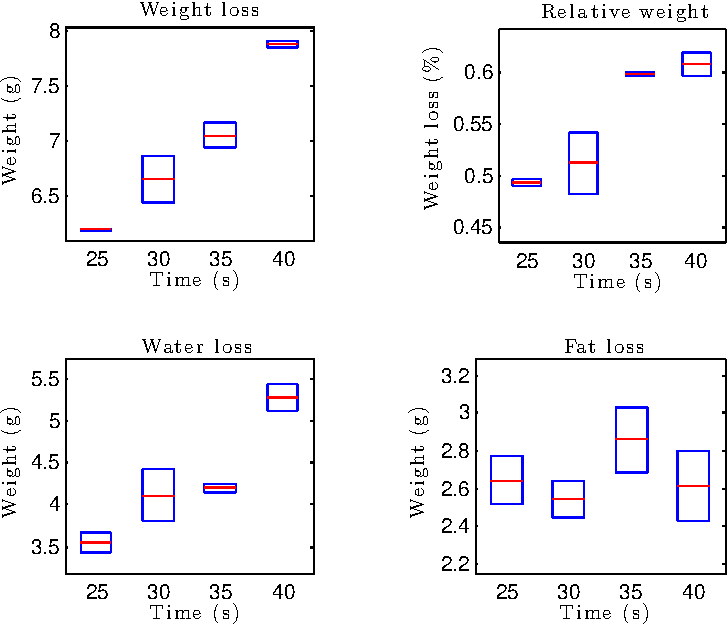
\includegraphics[width=0.5\textwidth]{thick_bacon}}\qquad
\subfloat[Regular bacon]{\label{fig:regular_bacon}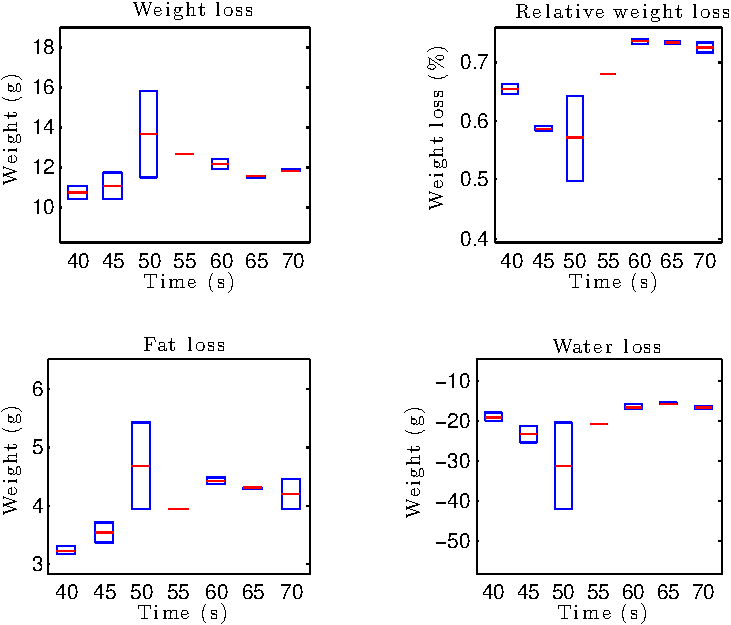
\includegraphics[width=0.5\textwidth]{regular_bacon}}
\caption{Schematic representation of measured data}
\label{fig:baconplot}
\end{figure}

\section{Results and discussion}

As can be seen in \cref{fig:thick_bacon} the water loss from 30-35 seconds is
approximately constant, while the fat loss is increasing on the same
time interval. This shows that around 30-35 seconds fat starts to melt,
``stealing'' heat from the water, this is in correspondence with weight loss as
a function of time. The fat loss continues to increase linearly
up to about 50 seconds, see \cref{fig:regular_bacon}. After 50
seconds the fat loss stabilizes, indicating that no more fat can be lost, and
that further baking time results in burnt bacon. $\\$

These results agree with expectations that the weight loss would
stabilize after a critical time, something that is clearly demonstrated in
\cref{fig:baconplot}. It is worth commenting that the big variation in
\cref{fig:regular_bacon} for $t = 50$s is due to one enormous (relative to the
others) bacon slice.

 %Kap. 5
	\include{resultats_numerics} %Kap. 6
	\chapter{Conclusion}
\section{Discussion of the results}

\section{Conclusion}
The performed numerical simulations and experiments with bacon preparation
in a microwave oven gave satisfactory results so far as they were implemented. 
The numerical simulations of the heat equations gave reasonable results in agreement
with experiments. An implementation of the transport equation would have been
more satisfactory, and is suggested as a possibility for future work in this
direction. The experiments performed suggest that the fat transport is
complicated, and that gravity is not dominating the flow. 


	%Kap. 7
=======
	\chapter{Innledning}
\fancyhead{}
\section*{Innledning}
Denne rapporten er skrevet i sammenheng med faget TMA4850 Eksperter i Team våren
2011 av gruppa Fu\th ark. Rapporten har som mål å vise utviklingen til gruppa
og gruppas dynamikk gjennom prosjektet, og å bevisstgjøre medlemmene på
prosessene som har funnet sted langs veien.

Rapporten er delt inn i seks kapitler. \emph{Innledningen} leser du nå.
\emph{Presentasjon av gruppens medlemmer} tar nettopp for seg å presentere
gruppens medlemmer, deres faglige bakgrunn, erfaring med gruppearbeid og hvordan
resten av gruppa ser på medlemmet. \emph{Teori} tar for seg de forskjellige
teoretiske modellene for gruppearbeid og gruppedynamikk, og setter dem inn i en
relevant kontekst. Videre beskrives \emph{Oppstart og utvikling} i arbeidet med
prosjektet og prosessen, og til slutt drøftes \emph{Analyse av gruppearbeidet}
der vi peker på sammenhenger mellom teori og praksis i vår gruppe, ser på
gruppas bruk av regler og teori, og ser på hvordan dette stemmer med
virkeligheten. Det siste kapittelet presenterer vår \emph{Konklusjon}.
 	%Kap. 1
	\chapter{Teori}
\section{Schwarz - gruppeteori}
\subsection{Effektivitet}


Flere faktorer påvirker en gruppes effektivitet; har gruppen et klart mål? Er
medlemmene enig om arbeidsmetode, og er de motiverte for den? For å forenkle
jobben som fasilitator, og/eller gi gruppemedlemmene mulighet til å påvirke
effektiviteten selv, har Schwarz utviklet en ``modell'' for hva som gjør grupper
effektive. Det er verdt å merke seg at Schwarz siterer George Box i
introduksjonen til kapittelet: ``All models are wrong; some are useful''.

Schwarz setter opp tre kriterier for effektivt gruppearbeid:

\begin{itemize}
\item[\textsc{Ytelse}] Tjenesten eller produktet gruppen leverer møter (eller overgår)
	forventningene og/eller kravene til de som skal bruke/motta/evaluere
	tjenesten.
\item[\textsc{Prosess}] Prosessene bak utførelsen av arbeidet vedlikeholder, eller
forbedrer, gruppemedlemmenes mulighet til å samarbeide på videre
arbeidsoppgaver.
\item[\textsc{Personlig}] Gruppeerfaringen skal bidra til personlig vekst og god
selvfølelse blant medlemmene.
\end{itemize}

Disse kriteriene er avhengige av hverandre, og for at en gruppe skal være
effektiv må den møte alle tre kritierer. Bryter gruppen på ett punkt vil det
påvirke de andre, for eksempel: Hvis en gruppe håndterer konflikter på en slik
måte at tilliten mellom medlemmene avtar, vil det på sikt føre til at medlemmene
holde informasjon tilbake fra resten av gruppen. Dette vil igjen føre til at
nøkkelinformasjon ikke er tilgjengelig for samtlige gruppemedlemmer, og gruppen
vil bli ineffektiv.

Videre beskrives måter en gruppe kan sikre seg effektivitet. En effektiv gruppe
håndterer konflikter i det åpne, og baserer seg på antagelsen om at hver enkelt
medlem er sterk nok til å takle negativ tilbakemelding. I tillegg er det viktig
å ikke bare løse konflikten, men også finne ut hva som forårsaket den. $\\$

Det er også viktig at man kommuniserer på en slik måte at mottaker og avsender
har samme oppfatning av hva som blir sagt. Altså må man passe på at det man sier
blir oppfattet korrekt, dette kan oppnås ved å ikke bare avsløre hva du har
funnet ut, men også \emph{hvordan} du kom til den konklusjonen. Ved å bruke
denne kommunikasjonsmetoden oppmuntres andre til å finne ``hull'' i logikk og
løsningsmetode, i tillegg til at mottaker blir tvunget til å komme med

motargumenter. Effektive grupper tester også ut sine antagelser, det vil si at
dersom et gruppemedlem sier noe svarer mottaker med å fortelle hva han/hun tror
den andre mente. Man minimerer da muligheten for misforståelser og videre
frustrasjon. $\\$

Effektive grupper må også ha klare definerte rammer for oppgaven som skal løses, 
det er også viktig at hvert gruppemedlem kjenner (og klarer å uttrykke) denne
oppgaven. Gruppen må også sørge for at hvert medlem har en klar oppfatning av
sin egen rolle i oppnåelsen av gruppeoppgaven. I samme omgang bør det sørges for
at beslutningsprosesser og hierarki i gruppen er klart definert og forstått. $\\$

En enkel, men god, måte og oppnå alle disse punktene på, er å bruke endel tid i
starten på å få til en bra samarbeidskontrakt. Der hvor tema som lederskap,
problemstilling, beslutningsmønstre, oppgavefordeling osv. kan innlemmes. Se
\cref{sec:kontrakt}. Schwarz har kokt alt dette ned til 9 grunnregler som skal sørge for
gruppeeffektivitet. Se \cref{sec:grunnregler}.
\clearpage

\subsection{Grunnregler}
\label{sec:grunnregler}
For å sikre effektivt gruppearbeid har Schwarz \cite{schwarz} etablert et sett
med grunnleggende regler (\cref{tab:grunnregler}), dette sørger for at gruppa har et enkelt og
oversiktlig oppslagsverk og vise til, for eksempel ved diskusjoner. I tillegg er
det en god pekepinn på punkter som bør være i samarbeidskontrakten.
\begin{center}
\begin{table}[ht!]
\begin{tabular}{r l}
1. & Test antagelser og slutninger \\
2. & Del \emph{all} relevant informasjon \\
3. & Bruk spesifikke eksempler og bli enig om betydning av fremmedord \\
4. & Forklar resonnement og intensjon. \\
5. & Fokuser på interesser, ikke posisjon. \\
6. & Kombiner støtte og granskning \\
7. & Utform fremgangsplaner og tilbakemeldingsmåter i plenum. \\
8. & Etabler metode for å ta opp ``ikke-tema''. \\
9. & Bruk et beslutningsmønster som sørger for nødvendig engasjement. \\
\end{tabular}
\caption{Schwarz' regler for effektive grupper}
\label{tab:grunnregler}
\end{table}
\end{center}

\section{Johnson \& Johnson}
\subsection{Gruppedynamikk}
Gruppedynamikk handler om den vitenskapelige studien av oppførsel i grupper.
Adferd i grupper, og forståelsen av den, er essensielt, da mennesker i all
hovedsak er gruppedyr, det være seg i familien, blant venner eller på jobb. Det
første som må læres er; ``hva er en gruppe?''. Spørsmålet er vanskeligere enn
man skulle tro, og Johnson \& Johnson (J\&J) \cite{jj} viser til at sosiologene
fortsatt ikke er enige om én definisjon. Likevel kan man si at en gruppe er en
samling av minimun to personer, som relaterer med hverandre ansikt til ansikt.
Samtlige individer i gruppa er også klar over at de er avhengige av de andre for
å få jobben gjort, i tillegg til at det er klart definert \emph{hvem} som er med
i gruppa. $\\$

J\&J påstår videre at en gruppes produktivitet er avhengig av fem
basiselementer:
\begin{itemize}
\item[$1.$] Positiv avhengighet blant medlemmer.
\item[$2.$] Individuell ansvarsfølelse.
\item[$3.$] Fremmende interaksjon.
\item[$4.$] Fungerende sosiale antenner.
\item[$5.$] Gode gruppeprosesser.
\end{itemize}
Hvis man i tillegg skal sørge for at gruppen er effektiv må gruppemedlemmene
\textbf{(1)} Sørge for at gruppens felles mål anvender hvert medlems
individuelle kompetanse, \textbf{(2)} forsikre at kommunikasjon mellom hverandre
er nøyaktig og forstås korrekt, \textbf{(3)} etablere lederskap og/eller
passende innflytelse, \textbf{(4)} implementere beslutningsmønstre som sørger
for at samtlige medlemmer kommer med innslag, i tillegg til at hver enkelts
resonnement og konklusjon er åpne for evaluering og analysering, \textbf{(5)}
etabler metoder for å håndtere konflikter konstruktivt.$\\$

\subsection{Å verdsette ulikheter}
Det er uunngåelig at en gruppe vil bestå av personer med ulike egenskaper. Det
være seg faglige, personlige, kulturelle, religiøse, etniske og så videre.
Det er viktig å sørge for at ulikhetene blant gruppemedlemmene kulminerer i noe
positivt, Johnson \& Johnson presenterer ulike måter man kan forsikre dette på.
Man må forsikre at det mellom gruppemedlemmene er en stor grad av positiv
avhengighet av hverandres arbeid. Gruppen må også forsøke å etablere en felles
gruppeidentitet som alle medlemmene kan samle seg bak, denne må være basert på
flertallets verdier. I oppstartsfasen er det viktig at det brukes tid på å lære
om forskjellene mellom medlemmene, et slikt enkelt grep kan kartlegge ulike
måter og ordlegge seg på (eksempelvis i ulike kulturer), som kan forhindre
miskommunikasjon og misforståelser på et senere stadium. $\\$

Det er også viktig at det etableres gode rutiner for konflikthåndtering, noe som
helt sikkert vil oppstå i heterogene grupper. Konfliktene bør håndteres slik at
gruppa får klarhet i hva som forårsaket uenigheten, og hva som ble gjort for å
løse den. Bruk også tid på at gruppemedlemmene skal bli kjent med hverandre på
et personlig nivå, på denne måten forsikrer man at diskusjonene mellom personene
i gruppa blir friere og bedre.

\section{Wheelan}
ubsection{Effective teammedlemmer}

Wheeland beskriver gruppemedlemmer's oppførsel og holdninger i effektive grupper. En viktig del ved å være en effektiv gruppemedlem består i å vurdere sin egen oppførsel og holdning og måten man kommuniserer med gruppa på. Teorien er presentert i form av retningslinjer. 

\begin{itemize}
\item[1.] Ikke skyld på andre for gruppas problemer
\item[2.] Vær engasjert når gruppa setter mål, roller og avklaring av oppgaver
\item[3.] Vær for en åpen kommunikasjonsstruktur der alle medlemmer deltar og blir hørt 
\item[4.] Ha en riktig fordeling mellom diskusjon av oppgaven og støttende kommunikasjon
\item[5.] Bruk en effektiv måte å løse oppgaver på, og en effektiv måte å ta avgjørelser
\item[6.] Lage normer som støtter produktivitet, innovasjon og frihet til å uttale seg
\item[7.] Bidra med normer som forfremmer produktivitet
\item[8.] Forfremme gruppearbeid
\end{itemize}

Punkt 1 kaller Wheeland for ''the fundamental attribution error'', fordi vi ofte tilskriver andres holdninger til personlige trekk uten å ta andre faktorer i betraktning. For eksempel kan vi skylde på sjefen for dårlige resultater uten å ta i betraktning budsjettrestriksjoner, og dårlig gruppesammarbeid. En gruppe blir ikke effektiv før alle tar ansvar for gruppa's samarbeid og produktivitet. \\

Punkt 2 dreier seg om å være klar over hva som foregår i gruppearbeidet. Hvis man ikke forstår hva som foregår, må man våge å spørre. Å stille spørsmål til hele gruppa vil føre til en rikere diskusjon og vil klargjøre ting for alle gruppemedlemmer. \\

Punkt 3 tar opp problemet med at medlemmer i gruppa ikke tør å si det de mener fordi de ofte klassifiserer andre i gruppa, og ut i fra det angir dem høyere eller lavere status. Disse medlemmene kan bli ignonert i gruppa, noe som fører til at gruppa blir mindre produktiv. En måte å sikre at alle blir hørt på er så enkelt som å ta en runde rundt bordet for å høre hva hver og en har å si. \\

Punkt 4 handler om oppgaveorientert diskusjon i gruppen. Forskning tyder på at suksessfulle grupper bruker om lag 70-80 \% av tiden sin til å diskutere oppgave og mål. Men ofte hender det at gruppa går seg bort i en lang diskusjon om noe annet. \\

Punkt 5 diskuterer effektive måter for oppgaveløsning og det å ta beslutninger. Det nevnes fire steg som kan følges: Å innse problemet, diagnotisere problemet, ta beslutningen, og akseptere og gjennomføre beslutningen. I praksis består de to første stegene i å planlegge strategier for å løse problemet. Når man så skal ta en beslutning er det ikke noe klart svar på hvilken beslutningsmåte som er best, men gruppa skal velge en beslutningsmåte der alle medlemmer kan akseptere beslutningen.  \\

Punkt 6 handler om gruppas avtale. Hvis gruppas medlemmer bare er middelsmådige enige, blir resultatet også middelsmådig. Hvis medlemmene derimot er enige om å gjøre en best mulig jobb og løse problemer på best mulig måte, er det større sannsynlighet for at resultatet blir bra. Frihet til å uttale seg er nevnt i punkt 3. \\

Punkt 7 dreier seg om normer, dvs. regler om medlemmenes oppførsel og hva som skal gjøres. Normer er nødvendige for å samordne gruppas arbeid mot et felles mål. Spesielt er normer viktige når medlemmene er uenige i hvordan ting skal gjøres. \\

Punkt 8 diskuterer karaktertrekk ved god gruppesamarbeid. Disse er bl.a. god kommunikasjon, vennlig atmosfære, stor innsatsvilje, og stor grad av arbeidsfordeling.

\section{Kommunikasjonsteori}
%look at patterns of group communication and the variables that influence communication effectiveness
%
For at ei gruppe skal kunne fungere effiktivt, er det viktig at medlemmer klarer å kommuniserer enkelt og effektivt. Særlig i en tværrfaglig gruppe er det viktig at medlemmer er effektive i å formidle videre den informasjonen dei innehar. (Då løysninga av problemet i stor grad avhenger av evnen til gruppa har til å flette sammen informasjon som fleire medlemmer innehar, er det viktig at mottakeren av informasjon sitter igjen med det samme bilde som sender prøver å formidle.) Det er derfor viktig å he ein grunnleggende forståelse for gruppekommikasjon.
For å forstå gruppekommunikasjonen i eit team, er det to ting som er viktige å sjå nærmere på; kommunikasjonsmønsteret/ kommunikasjonsnettverk og kommunikasjonseffektiviteten. Ved kommunikasjonsmønsteret meiner me her kven som kommunniserer med kven. Me kan her snakke om ein einvegskommunikajsone, der lederen adresserer gruppa, eller ein toveiskommunikasjon, som t.d. myldring blant gruppemedlemmer. Kommunikasjonseffektiven er her definert som evnen til å formidle ein beskjed på ein slik måte at mottakeren tolker beskjeden slik som sender sjølv har tenkt.
Variable som kan verke inn på gruppe kommunikasjonen er normer på gruppa, konkurranse innad i gruppa, arbeidsmiljet, sittearrangementer og humor innad i gruppa.
\\
\section{Roller}
«I grupparbete spelar rollerna roll» (Stefan Jern, (1))\\

«Ei rolle kan defineres som ein spesiell type særegenhet, som definerer din plass på gruppa». Ei gruppe består av ulike individ som kvar har sine særegenskaper. Desse personlige trekka er ein faktor som er med på å definere kva rolle eit medlem vil spele på gruppa.  Når ei gruppe går sammen, byggjes det forventninger til rolla dei andre vil ha på gruppa utfrå inntrykket dei får av individet. Dine egne forventninger og gruppas forventninger til di rolle er i stor grad med på å forme den rolla du vil ha i gruppa vidare. I eit gruppesamarbeid med flat struktur snakker me her om informelle roller. Informelle roller er roller som vekser fram gjennom samspelet i gruppa. Informelle roller i eit gruppesamarbeid kan i hovudsak deles i to roller; instrumentelle roller og sosio-emosjonelle roller. 
\\
\\
I Robert-Bales likevektsteori statuerer han viktigheten ved ein balanse mellom arbeidsoppgåver og sosial-emosjonelle aktiviteter i effektive grupper. I effektive grupper ser ein derfor ofte at eit medlem trer inn i rolla som instrumentell leder, mens ein annan trer inn i rolla som sosial-emosiell leder. Kjenneteiknet på ein oppgåve-leder er at det er ofte han som setter igang aksjoner for å sikre at målet til gruppa blir nådd (oppgåveretta aksjoner), mens den sosiall-emosielle lederen setter igang aksjoner for å oppretthalde og forbedre interrelasjonene i gruppa (relasjonsretta aksjoner).
\\
\\
I ein flatstrukturert gruppe er lederrollen ofte avhengig av situasjoner gruppa møter. Situsjonsbetinget lederskap er definert som delt lederskap blant gruppemedlemmer der medlemmene varierer oppførselen etter kva funksjon gruppa treng til ein kvar tid. Ein funksjon er ein aksjon som blir sett igang for å sikre effektiviteten i gruppa, og kan vera enten oppgåveretta aksjoner og relasjonsretta/samholdsretta aksjoner. 

Benne og Sheat beskreiv i 1948, tretten instumentelle roller. Her tar eg for meg nokon av dei som var mest fremmtredene i vår gruppe; initiativtakeren, informasjonssøkaren, informasjonsgiveren, meiningsøkjaren, meiningsgivaren, diagnostikeren, samordnaren, opplysnaren, energigiveren og kritikkeren. Desse er alle viktige roller på gruppa. 

Meiningsøkjaren spelar ein viktig del på gruppa ved at han innbyr til beslutningstaking, og legg grunnlaget for individ til å fremleggje sin vurdering av framlagte fakta. Diagnostikeren er den analyserende parten på gruppa, som tar opp problemer/utfordringer ved oppgåve, og eventuelt leder gruppa i ei ny retning. Samordnaren derimot bidrar ved å samkjøre gruppas arbeid og flette dei samman til ein heilhet.

Benne og Sheat satt og opp åtte sosio-emosjonelle roller i ei gruppe; oppmuntraren, harmoniseraren, spenningoppløseren, kompromisten, målvakten, kjenslertolken, normsetteren og følgeren. Ein målvakt verkar som ein slags ordstyrar, som øker kommunikasjonen ved å bremse pratmakerene og passe på at alle kjem til ordet. Desse rollene kan flukturerer mellom medlemmene på gruppa, men ofte ser ein at eit individ påtar seg nokon roller med høgare frekvens.
		%Kap. 2
	\chapter{Numerikk}

\section{Von Neumann-analyse av Crank-Nicolson-skjemaet}

\begin{equation}
\frac{\partial u}{\partial t} = \alpha\frac{\partial^2u}{\partial^2x}
\label{varmelikn}
\end{equation}

\noindent Ved å anvende Crank-Nicolson oppnås følgende iterasjonsskjema

\begin{equation}
u_i^{n+1} = u_i^n\left(1-2D\right)+D\left(u_{i+1}^{n+1}-2u_i^{n+1}+u_{i-1}^{n+1}\right) + D\left(u_{i+1}^n + u_{i-1}^n\right)
\end{equation}
\begin{equation}
D = \frac{1}{2}\frac{\alpha\Delta t}{(\Delta x)^2}
\end{equation}

\noindent Innfører tilnærmelsen $u_j^n \approx E_j^n$ hvor $E_j^n = G^ne^{i\beta
x_j}$, her er $n$ en potens. Innsatt i \cref{varmelikn}:

\begin{equation*}
G^{n+1}e^{i\beta x_j} = G^ne^{i\beta x_j}\left(1-2D\right) + G^{n+1}D\left(e^{i\beta x_{j+1}} - 2e^{i\beta x_j} + e^{i\beta x_{j-1}}\right) + G^nD\left(e^{i\beta x_{j+1}} + e^{i\beta x_{j-1}}\right)
\end{equation*}

\noindent Hvis vi deler $(3)$ på $G^ne^{i\beta x_j}$ og benytter at $x_{j+1} \approx x_j + h$ får vi
\begin{eqnarray*}
G\left[1-D\left(2\cos{\beta h} - 2\right)\right] &=& 1 - 2D\left(1-\cos{\beta h}\right) \\
\cos{\beta h} &=& \frac{1}{2}\left(1-\sin^2{\frac{\beta h}{2}}\right) \\
G\left(1+4D\sin^{2}{\frac{\beta h}{2}}\right) &=& 1 - 4D\sin^2{\frac{\beta h}{2}} \\
G &=& \frac{1-4D\sin^2{\frac{\beta h}{2}}}{1+4D\sin^2{\frac{\beta h}{2}}}
\end{eqnarray*}

\noindent Vi vet at den maksimale verdi av $\sin^2{x}$ er $1$, og at iterasjonsskjemaet er stabilt dersom $|G| \le 1$, innsatt:

\begin{equation}
|G| = \left|\frac{1-4D}{1+4D}\right|
\end{equation}

\noindent Verdt å observere at så lenge $D > 0 \ \Rightarrow \ |G| \le 1$, slik at Crank-Nicolson-skjemaet er \emph{ubetinget stabilt} 

\subsection{Truncation error}

The Crank-Nicholson method is based on the trapezoidal rule. From the trapezoidal rule the truncation error is represented by

\begin{equation*}
\int_0^k f(t) dt = \frac{1}{2} k (f(0) - f(k)) -\frac{1}{12} k^3 f''(\frac{k}{2}) + ...
\end{equation*}

\noindent Using the formula

\begin{equation*}
	u(x_m,t_{n+1}) - u(x_m,t_n) = \int_{t_n} ^{t_{n+1}} u_t(x_m,t) dt
\end{equation*}

and approximating the integral by the trapezoidal rule, and abbreviate the notation $u_m^{n+1/2} = u(x_m,t_n+\frac{1}{2} k)$, one obtain

\begin{eqnarray*}
u_m^ {n+1} &=& u_m^ n + \frac{1}{2} k(\partial_t u_m^n + \partial_t u_m^{n+1}) - \frac{1}{2} k^3 \partial_t ^3 u_m^{n+\frac{1}{2}} \\
		   &\stackrel{\text{\tiny heat eq.}}{=}&  u_m^ n + \frac{1}{2} k(\partial_x^2 u_m^n + \partial_y^2 u_m^n + \partial_z^2 u_m^n + \partial_x^2 u_m^{n+1} + \partial_y^2 u_m^{n+1} + \partial_z^2 u_m^{n+1}) - \frac{1}{2} k^3 \partial_t ^3 u_m^{n+\frac{1}{2}}
\end{eqnarray*}

Discretizing the double derivative with central differences, and denoting the step sizes in $x, y, z$ direction by $h, f, g$ respectively, gives

\begin{eqnarray*}
u_m^{n+1} &=&  u_m^ n + \frac{1}{2} k(\frac{1}{h^2}\delta_x^2 u_m^n + \frac{1}{f^2}\delta_y^2 u_m^n + \frac{1}{g^2}\delta_z^2 u_m^n + \frac{1}{h^2}\delta_x^2 u_m^{n+1} + \frac{1}{f^2}\delta_y^2 u_m^{n+1} + \frac{1}{g^2}\delta_z^2 u_m^{n+1}) \\
 		  &&- \frac{1}{2} k (\frac{1}{12}h^2\partial_x^4 u_m^n + \frac{1}{12}g^2\partial_y^4 u_m^n \frac{1}{12}f^2\partial_z^4 u_m^n + \frac{1}{12}h^2\partial_x^4 u_m^{n+1} + \frac{1}{12}g^2\partial_y^4 u_m^{n+1} \frac{1}{12}f^2\partial_z^4 u_m^{n+1} ) \\
 		  &&- \frac{1}{2} k^3 \partial_t ^3 u_m^{n+\frac{1}{2}} \\
 		  &=& u_m^n + \frac{r}{2}(\delta_x^2 u_m^n + \delta_x^2 u_m^{n+1}) + \frac{p}{2}(\delta_y^2 u_m^n + \delta_y^2 u_m^{n+1}) + \frac{q}{2}(\delta_z^2 u_m^n + \delta_z^2 u_m^{n+1}) + \tau_m^n
\end{eqnarray*}

where $r = k/h^2$, $p = k/f^2$, $q = k/g^2$, and $\tau_m^n$ is the truncation error times $k$. The expression for $\tau_m^n$ is

\begin{equation*}
\tau_m^n = -\frac{1}{12} k^3 \partial_t^2 u_m^{n+\frac{1}{2}} - \frac{1}{12} k h^2 \partial_x^4 u_m^{n+\frac{1}{2}} - \frac{1}{12} k g^2 \partial_y^4 u_m^{n+\frac{1}{2}} - \frac{1}{12} k f^2 \partial_z^4 u_m^{n+\frac{1}{2}}
\end{equation*}

where we have used $\frac{1}{2}(\partial_x^4 u_m^n + \partial_x^4 u_m^{n+}) = \partial_x^4 u_m^{n+\frac{1}{2}} + O(k^2)$. Hence, the truncation error is 

\begin{eqnarray*}
\frac{\tau_m^ n}{k} &=& -\frac{1}{12} k^2 \partial_t^2 u_m^{n+\frac{1}{2}} - \frac{1}{12} h^2 \partial_x^4 u_m^{n+\frac{1}{2}} - \frac{1}{12} g^2 \partial_y^4 u_m^{n+\frac{1}{2}} - \frac{1}{12} f^2 \partial_z^4 u_m^{n+\frac{1}{2}}\\
					&=& O(k^2 + h^2 + g^2 + f^2)
\end{eqnarray*}	%Kap. 3
	\chapter{Implementation}

\section{Tools}

The programming language chosen to implemented the system was c++.
The arguments leading to this choice was:

\begin{itemize}
\item Most of the group members had some earlier experience with the language.
\item It allows for a high level of abstraction without loosing control of the
underlying hardware.
\item The code can be easily parallelized for shared memory machines using OpenMP.
\item Many libraries exist for c++ that implements highly optimized linear algebra
functionality.
\end{itemize}

Other languages cosidered where Matlab and c.

The tool chosen to visualize the resulting data was gnuplot and ffmpeg. Writing a
program using OpenGL was considered, but dismissed on the grounds of beeing too time consuming.

\section{Program design}

The program mainly consist of three parts:

\begin{itemize}
\item C++ implementation of Linear algebra functionality of the discrete equations.
\item C++ implementation of the conjugate gradient method for solving the
equations described.
\item Bash script for generating plots and and movie of the generated data.
\end{itemize}

The Bash script is not discussed in further detail as it can be considered simple.

\section{The physical system}

The main task of the physical system is to implement a matrix-vector multiplication
procedure for the heat equation and a method of calculating the heating properties of
a microwave.

\subsection{Partitioning of the problem}

\subsection{Updating alpha and beta values}

\subsection{Calculating the distribution of the microwave effect}

\subsection{The matrix-vector multiplication procedure}

\section{The conjugate gradient method as an iterative algorithm}


 %Kap. 4
	\chapter{Eksperimenter}
\section{Eksperimenter}
\lipsum[1-3]
 %Kap. 5
	\chapter{Numerikkresultater}
\section{Numerikkresultater}
\lipsum[1-3]
 %Kap. 6
	\chapter{Konklusjon}
Allerede på de første landsbydagene la vi merke til at vi hadde hatt flaks med
gruppesammensetningen. Alle gruppas medlemmer var innstilte på å gjøre en god
jobb, og vi merket fort at stemningen i gruppa var god. På starten var vi
noe negativt innstilt til jobbing med prosess. Vi så ikke på forhånd nytten
av å dedikere spesifikk tid til å arbeide med teambygging, og mente at teambygging
ville skje naturlig dersom vi bare fikk jobbe med prosjektet. \\

Etterhvert som vi fikk jobbet noen ganger med prosjekt og med prosess så vi at
prosessarbeidet har en klar nytteverdi. Øvelsene har i seg selv vært ganske
gode, selv om det har vært litt murring, hovedsaklig fordi det har avbrutt oss
mens vi var godt igang med prosjektarbeidet. Det at vi har arbeidet med prosess
samt å tilegne oss teori har ført til at grupperegler har ligget i bakhodet når
situasjoner har oppstått, slik at vi har tatt teorien i bruk i praksis, f.eks.
når vi .\\

Vi har også merket at vår tilegnelse av teorien har gjort det enklere å håndtere
situasjoner som har med gruppestruktur og gruppedynamikk å gjøre. Når man kan henvise
til en bestemt teori som underbygger argumenter for å omstrukturere er det
enklere å bli enige om et felles ståsted.\\

Den største endringen i gruppedynamikken så vi under framføringen i midten av
semesteret. Medlemmene fikk inntrykk av at de andre på gruppa var oppmerksomme
når man snakket, og at man fikk god støtte hvis man ble utrygg. Dette gjorde at
flere av medlemmene følte seg trygge nok til å improvisere med eksempler rundt
gruppas framgang. \\


	%Kap. 7
>>>>>>> 7058789ac84f4f187b361c86910142d6ef70d782

%Referanser:
	\bibliographystyle{plain}
	\bibliography{references.bib}

\end{document}

